% !TEX root = ../main.tex
% Approach
% Claims to support: RAGTAG, VTAG, fine-tuning, margin-based debiasing

\section{Approach}
\label{sec:03_approach}

\begin{figure}[t]
    \centering
    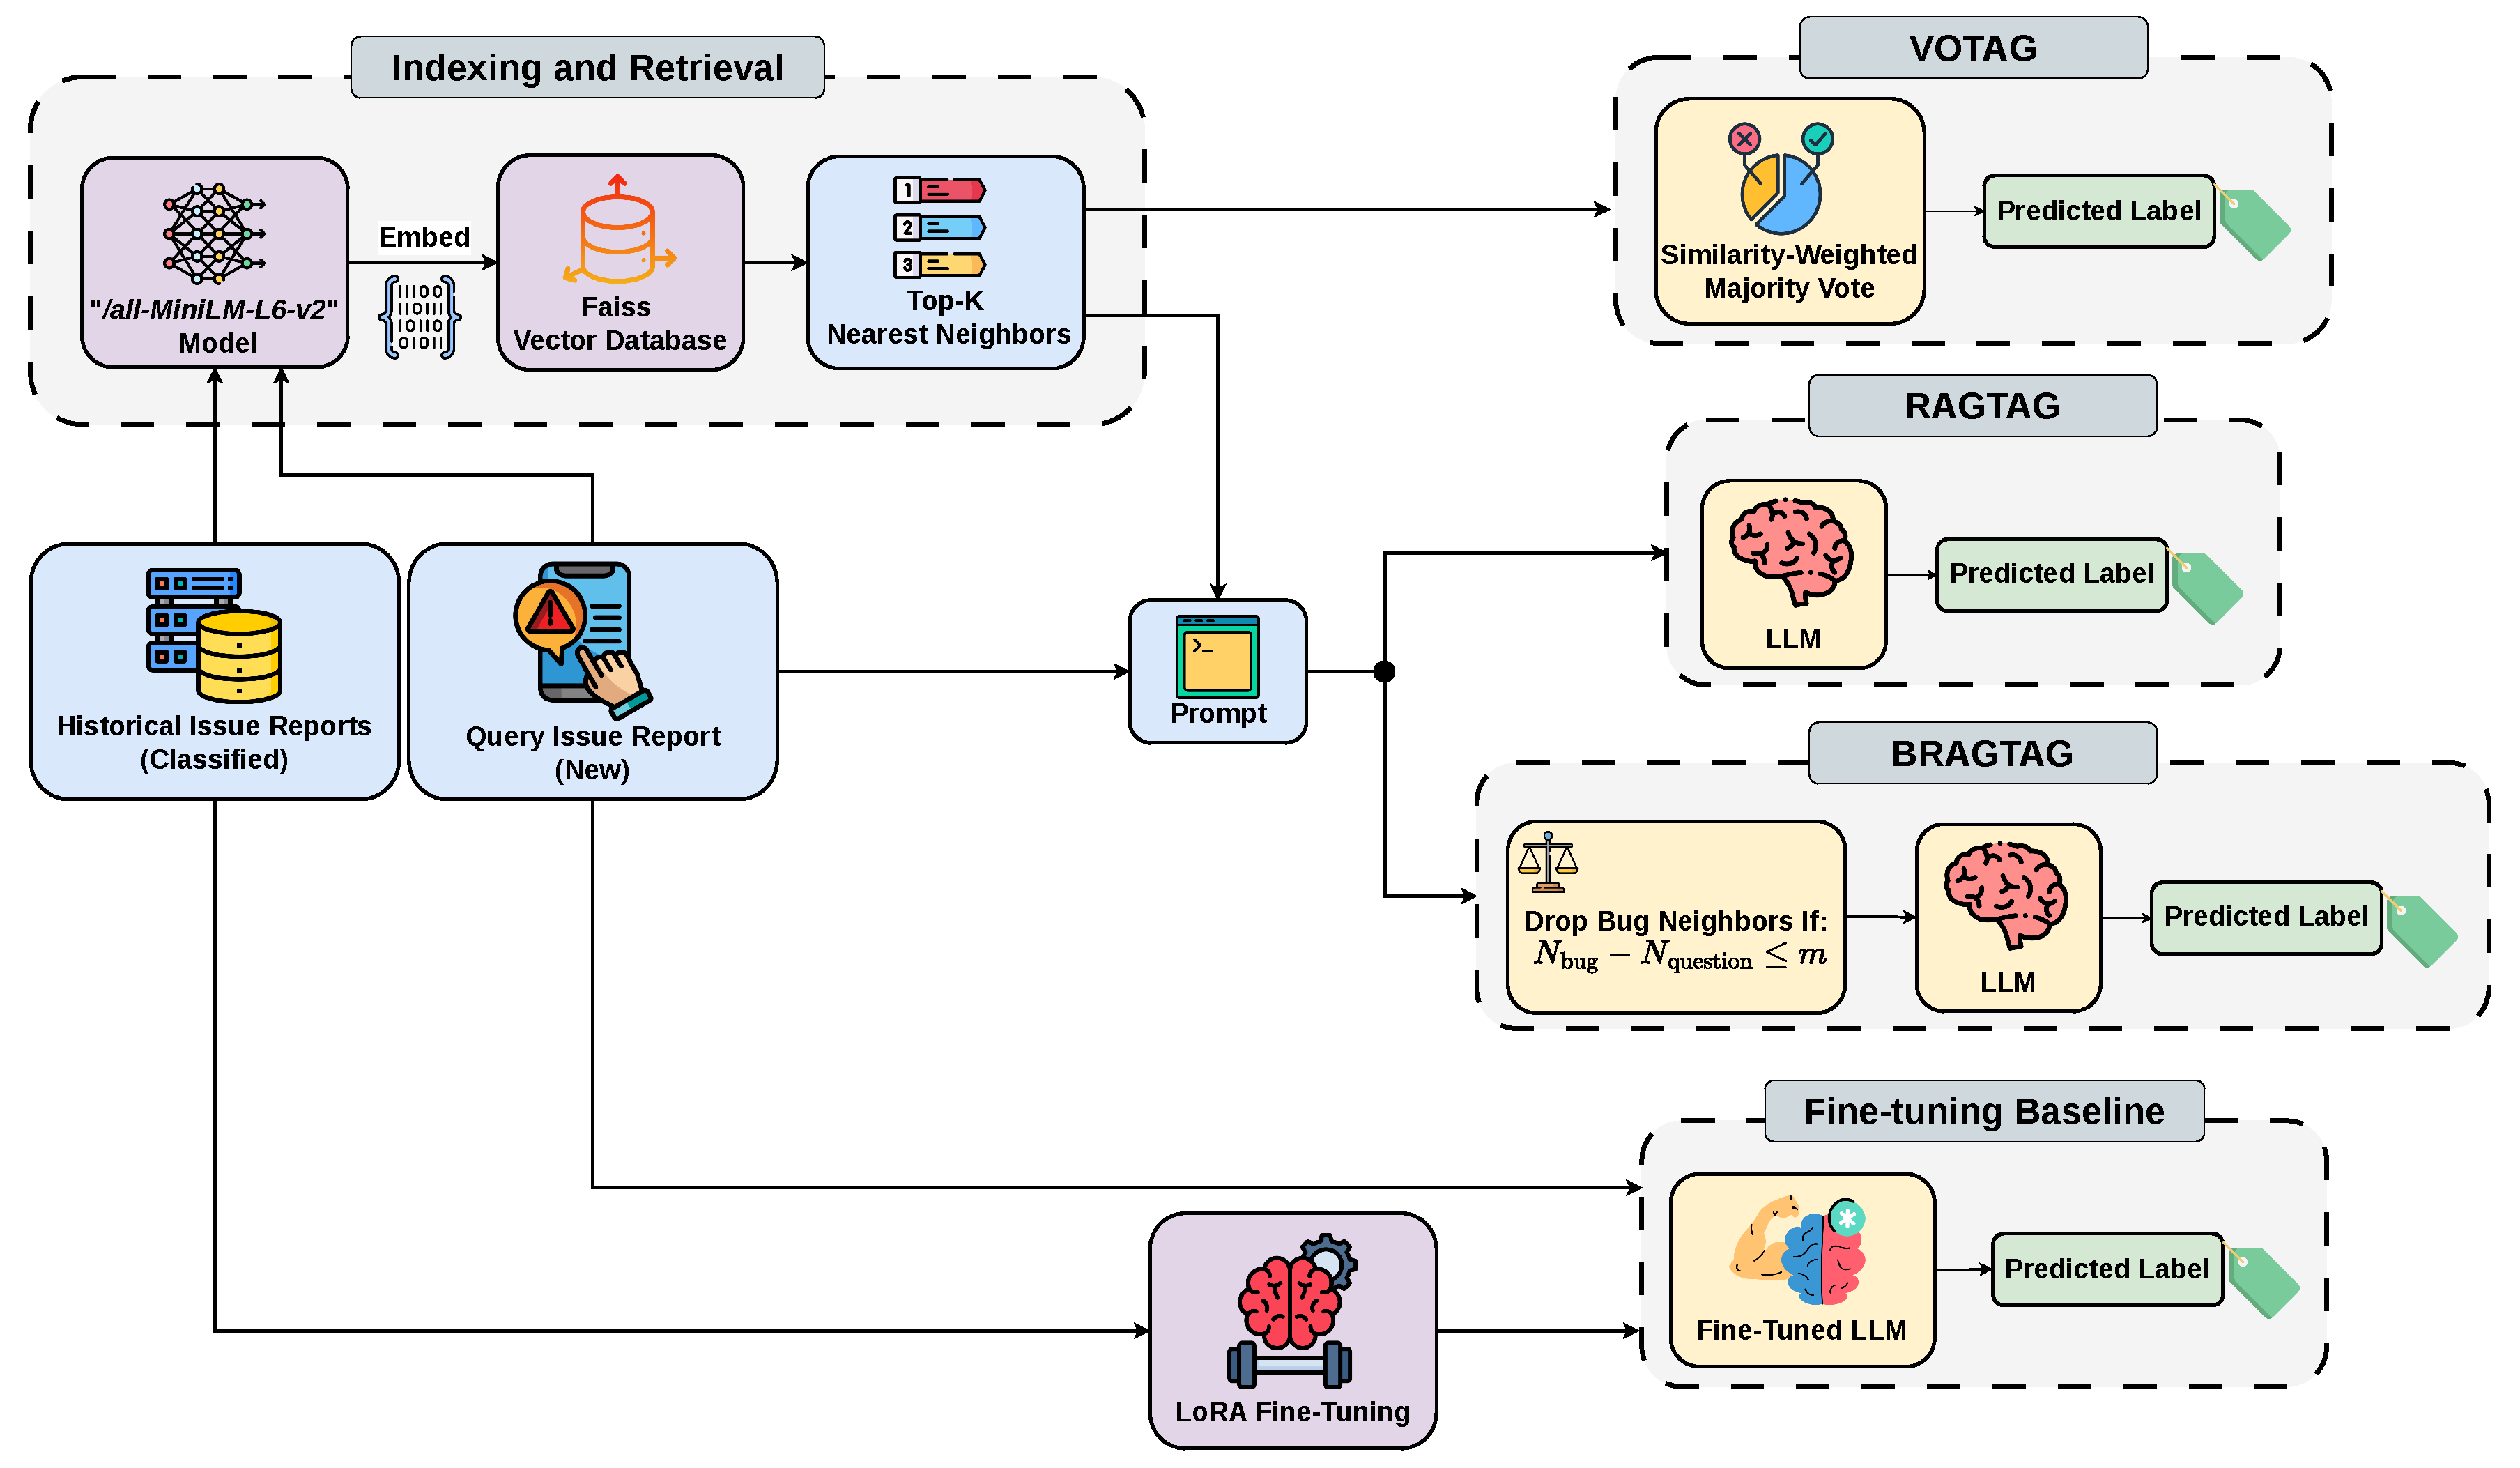
\includegraphics[width=0.85\linewidth]{figures/approach_diagram.pdf}
    \caption{Overview of the four IRC approaches evaluated in this paper: \votag, \ragtag, \bragtag, and the LoRA fine-tuning baseline.}
    \label{fig:approach-overview}
\end{figure}

In this section, we describe the intuition behind, and the full
implementation details of our three proposed retrieval-based IRC
methods (\votag, \ragtag, and \bragtag) as well as the faithful
reproduction steps of the established LoRA fine-tuning baseline~\cite{heo2025study,aracena2025applying}.
\Cref{fig:approach-overview} illustrates all four approaches to support
the explanations. The remainder of the section is
organized as follows: \Cref{sec:problem} explains the overall IRC
objective. \Cref{sec:retrieval} details the indexing and retrieval
pipeline shared by our three proposed retrieval-based methods.
\Cref{sec:approach-votag} presents \votag, our non-parametric method of classifying the query directly from its nearest neighbors. \Cref{sec:approach-ragtag} describes \ragtag, our few-shot prompting technique that presents the nearest neighbors as
classified examples in the prompt. \Cref{sec:approach-bragtag} elaborates on
\bragtag's balanced retrieval intervention on \ragtag. Finally,
\Cref{sec:finetune} details the faithful reproduction of the
fine-tuning baseline.

\subsection{Problem Formulation}
\label{sec:problem}
Given a query issue report, we classify it into only one of the three labels: \textit{bug}, \textit{feature}, or \textit{question}. Only the issue's title and description text are used for classification with no other signals from the issue tracker. The defined label space is adopted directly from prior IRC studies~\cite{aracena2024applyinglargelanguagemodels,aracena2025applying,izadi2022catiss,kallis2019ticket,antoniol2008bug}. 

\subsection{Indexing and Retrieval}
\label{sec:retrieval}
To prepare the issues for retrieval based on textual similarity, we first embed their textual content (i.e., \textit{title} + \textit{description}). We do not embed the issue labels. Instead, we retain them as metadata associated with each embedded issue. To generate the embeddings, we use the \texttt{all-MiniLM-L6-v2} model from the Sentence-Transformers library~\cite{reimers2019sentence}. We selected this model due to its lightweight architecture, fast performance, and effectiveness on issue report text~\cite{huang2025back}. The embeddings are then indexed using the Faiss vector database library~\cite{douze2025faiss}, which provides efficient high-dimensional similarity retrieval. At the retrieval stage, the query issue is first embedded with the same model. Next, Faiss calculates the cosine similarity of indexed issue reports to the query, and returns the top-K nearest neighbors, ordered by descending similarity.


\subsection{\votag}
\label{sec:approach-votag}
\votag is our proposed non-parametric retrieval IRC method. \votag uses the retrieval pipeline described in~\cref{sec:retrieval} to retrieve the top-K nearest neighbors of the query issue report, then predicts the final
label with a similarity-weighted vote on their labels. This approach follows the standard K-nearest-neighbor classification setup~\cite{cover1967nearest}, with neighbors weighted by their similarity to the query~\cite{dudani1976distance}.\footnote{Squared-similarity weighting and uniform majority were also evaluated, but were outperformed by similarity-weighted voting.} Formally, for a
query issue $q$ with retrieved neighbors $\{(n_i, l_i, s_i)\}_{i=1}^{K}$, where
$n_i$ is the $i$-th nearest neighbor with label $l_i$ and cosine similarity $s_i$ to $q$, the label is predicted by:
\begin{equation}
    \hat{y} = \operatorname*{arg\,max}_{c \in \mathcal{L}}
    \sum_{i=1}^{K} s_i \cdot \mathbf{1}[l_i = c],
    \label{eq:votag}
\end{equation}
where $\mathcal{L}$ is the label set and $\mathbf{1}[\cdot]$ is the indicator function. \votag breaks ties by returning the label of the most similar neighbor in the tied classes.



\subsection{\ragtag}
\label{sec:approach-ragtag}
\ragtag is our proposed retrieval-augmented few-shot prompting approach for
IRC. \ragtag uses the retrieval pipeline described in~\cref{sec:retrieval}
to retrieve the top-K nearest neighbors to the query issue, and present
them as classified examples to the LLM in a few-shot prompt. This enables
a more accurate classification, based on in-context
learning~\cite{brown2020language}. The choice to present the top-K nearest
neighbors as examples is based on two insights from prior research: First,
retrieval-based example selection outperforms random
selection~\cite{liu2022makes}. Second, the most similar neighbors tend to
share the same labels~\cite{cover1967nearest}; therefore, they are
informative for the classification.

We create the few-shot prompt in three parts. First, the system message frames the classification task and the label space. Second, the top-K nearest neighbors are listed in retrieval order (descending similarity), each formatted as \textit{title + description + label}. Finally, the query issue is appended to the end of the prompt, ensuring it receives high attention from the LLM~\cite{liu2024lost}. $K=0$ produces a zero-shot prompting baseline, similar to prior work~\cite{colavito2025benchmarking}.

We evaluate \ragtag at top-K values in $\{0, 1, 3, 6, 9, 12, 15\}$. Details
for the K value grid selection are provided in \cref{sec:rq1,sec:ragtag}. The maximum sequence length is set to 8,192 tokens.\footnote{Maximum sequence length is selected empirically. 8,192 tokens offered the best trade-off between classification accuracy and inference speed across our preliminary experiments.} Roughly 30\% of the
context quota is reserved for the query issue and 70\% for the
neighbors. If the neighbors exceed their overall quota, they are
truncated proportionally based on their length (longer neighbors get
more truncation). The query issue gets truncated if it exceeds its
budget as well. Truncation happens on the right side of the
description text, preserving all titles and labels (if any).


The LLM is instructed to generate the predicted label wrapped in XML tags (e.g. \texttt{<label>bug</label>}). The labels of the presented examples also follow the same format. This technique enables easy detection of the predicted label from the LLM's generation, and reduces variance in LLM outputs caused by prompt format sensitivity~\cite{sclar2023quantifying}. We use a regular expression to extract the predicted label. Unparseable outputs are marked as \textit{invalid}.

Finally, models are loaded with Unsloth\footnote{\url{https://unsloth.ai}} For memory efficiency, and the Temperature is set at 0.1 for deterministic classifications.

\subsection{Balanced \ragtag (\bragtag)}
\label{sec:approach-bragtag}
Our empirical evaluations in (\Cref{sec:ragtag}) reveal that \ragtag has the worst performance on the question label, and it frequently misclassifies true-question queries as bugs. Furthermore, LLM zero-shot results also show that the models are already biased towards predicting bug for true-question queries even before the examples are presented. Based on these insights, we hypothesize that presenting bug-labeled examples for true-question queries likely reinforces the question$\rightarrow$bug misclassification trend. To address this, we propose a more balanced retrieval intervention, called balanced \ragtag (\bragtag), that removes the bug-labeled neighbors whenever the query is a suspected question based on its nearest neighbors' label distribution. (\Cref{sec:ragtag}) shows that true-question queries retrieve almost balanced bug and question neighbors. Due to this balanced distribution, \bragtag should remove the bug-labeled examples from the prompt whenever bug neighbor count is within a small positive margin $m$ from the question neighbor count ($N_\text{bug} - N_\text{question} \le m$). The margin is empirically calibrated on a holdout validation set. The empirical motivations for \bragtag and its margin calibration are fully detailed in (\Cref{sec:ragtag})  



\subsection{LoRA Fine-Tuning Baseline}
\label{sec:finetune}
SOTA IRC approaches have achieved strong performance by supervised
fine-tuning of LLMs~\cite{heo2025study,aracena2025applying,
aracena2024applyinglargelanguagemodels}, using Low-Rank Adaptation
(LoRA)~\cite{hu2022lora}. In these studies, the
model is trained on labeled issue reports and predicts the labels for
unseen test issues. Each training example is formatted as an
instruction prompt which includes the issue's title and description
as input, and its label as output. At inference, the trained model
receives the test issue in the same format, and predicts the empty
label field. Regular expressions are used to extract the prediction
from the output, and unparseable outputs are marked as
\textit{invalid}. We use this established methodology as our fine-tuning baseline.

The LoRA rank and alpha are set to 16, with a learning rate of $2 \times 10^{-4}$ and the paged AdamW 8-bit optimizer. Training runs for 3 epochs with a per-device batch size of 1 and gradient accumulation steps of 16. The max sequence length is set to 2,048 tokens, which covers 94.9\% of the issues in our dataset. Issues that exceed this budget get truncated from the right side of their description text to fit.

Similar to \ragtag and \bragtag, the models are loaded with Unsloth\footnote{\url{https://unsloth.ai}} and the Temperature is set at 0.1.

